\documentclass[12pt, oneside]{report}

\usepackage[left=2.5cm, top=2.5cm, bottom=2.5cm, right=2.5cm]{geometry}

\usepackage[utf8]{inputenc}
\usepackage[T1]{polski}
\usepackage[polish]{babel}
\usepackage{hyperref}
\usepackage[table]{xcolor}
\usepackage{longtable}
\usepackage{graphicx}

\begin{document}  
\setcounter{tocdepth}{1} % + subsections
\thispagestyle{empty}
\begin{titlepage}
    \begin{center}

           \Large
	\textbf{Uniwersytet Jagielloński w Krakowie}\vspace{0.2cm}\\ Wydział Fizyki, Astronomii i Informatyki Stosowanej
               \vspace*{1cm}
               
         \vspace{3cm}
         \Large
          \textbf{Paweł Łabno}\\\vspace{0.5cm}
         \normalsize Nr albumu: 1138170\\
             \vspace{2cm}
        \Huge
        \textbf{Implementacja Sztucznej Inteligencji dla gry \textit{Wsiąść do Pociągu}}
      
        \vspace{1.5cm}
        \normalsize
        Praca magisterska\\
        na kierunku Informatyka Stosowana\\ \vspace{0.15cm}
        
        \vfill
        \vspace{2cm}
       \begin{minipage}{1\textwidth}
\begin{flushright}
Praca wykonana pod kierunkiem\\
<tytuł/stopień naukowy Imię Nazwisko>\\
<Instytut/Zakład>
\end{flushright}
\end{minipage}
        
        \vspace{2cm}
        \begin{center}
      Kraków 2018
        \end{center}
    \end{center}
\end{titlepage}

\newpage 
 \thispagestyle{empty}
\vspace{2.5cm}
\begin{flushleft}
\large \textbf{Oświadczenie autora pracy}\vspace{0.6cm}\\
\end{flushleft}

\noindent Świadom odpowiedzialności prawnej oświadczam, że niniejsza praca dyplomowa została napisana przeze mnie samodzielnie i nie zawiera treści uzyskanych w sposób niezgodny z obowiązującymi przepisami.\\

\noindent Oświadczam również, że przedstawiona praca nie była wcześniej przedmiotem procedur związanych z uzyskaniem tytułu zawodowego w wyższej uczelni.
\vspace{2cm}
\begin{center}
\begin{tabular}{lr}
................................~~~~~~~~~~~~~~~~~~~~~~~~~~~~~~~~~~~~~~&
.......................................... \\
{~~~~Kraków, dnia} & {Podpis autora pracy~~~~}
\end{tabular}
\end{center}
\vspace{5cm}
\begin{flushleft}
\large \textbf{Oświadczenie kierującego pracą}
\end{flushleft}

\noindent Potwierdzam, że niniejsza praca została przygotowana pod moim kierunkiem i~kwalifikuje się do przedstawienia jej w postępowaniu o nadanie tytułu zawodowego.
\vspace{2cm}
\begin{center}
\begin{tabular}{lr}
................................~~~~~~~~~~~~~~~~~~~~~~~~~~~~~~~~~~~~~~&
............................................ \\
{~~~~Kraków, dnia} & {Podpis kierującego pracą~~}
\end{tabular}
\end{center}
\vfill
\newpage
\tableofcontents
\newpage
\chapter{Wprowadzenie}
\section{Wprowadzenie do pracy}
Wraz z rozwojem możliwości technicznych komputerów człowiek szukał kolejnych zastosowań dla swojego wynalazku. Doskonałym celem do tego było sprawienie by życie człowieka stało się prostsze. Początkowo odbywało się to za pomocą przemyślanych i sprawdzonych algorytmów. Pojawiały się jednocześnie coraz bardziej skomplikowane problemy, dla których przygotowanie działającego algorytmu stanowiło wyzwanie. Na ratunek posłużyły sieci neuronowe, które po zaprojektowaniu wymagały odpowiednio przygotowanych danych uczących. \\ \\
Taka metoda pracy oraz podejmowania decyzji w ostatnich latach stała się coraz bardziej popularna i powszechnie wykorzystywana - np. w transporcie, finansach czy medycynie. Pojawiły się wreszcie próby wykorzystania sieci neuronowych w sytuacjach, dla których nie można z łatwością ocenić czy otrzymany wynik jest prawidłowy - gry. \\ \\ 
W mojej pracy chcę przygotować implementację sztucznej inteligencji dla gry \textit{Wsiąść do Pociągu} w oparciu o sztuczną sieć neuronową. 
\section{Definicja pojęć}
\paragraph{Gra} W literaturze pojawia się wiele definicji dla gry. Można uznać, że jest to czynność o rozrywkowym charakterze, w której uczestniczy jeden lub wielu graczy. Grę można również opisać jako model matematyczny charakteryzujący się określonymi zasadami oraz zbiorem możliwych operacji na tym modelu.
\paragraph{Teoria gier} W przypadku kiedy w rozgrywce uczestniczy więcej niż jeden gracz możemy rozważać zachowania każdego z uczestników. Można założyć, że każdy chce uzyskać jak najlepszy wynik dla siebie.
\paragraph{Klasyfikacja gry}
Gra \textit{Wsiąść do Pociągu} jest grą wieloosobową, niesymetryczną z niepełną informacją. 
\paragraph{Problem klasyfikacji}
W grze \textit{Wsiąść do Pociągu} pojawia się problem decyzyjny w postaci klasyfikacji. Klasyfikacja jest problemem przyporządkowania danego zestawu danych do jednej lub więcej klas ze zbioru co najmniej dwóch klas. \textit{Przeciwieństwo: Regresja}
\paragraph{Gra z niepełną informacją} 
Określenie gra z niepełną informacją oznacza, że gracze podejmują swoje decyzje nie wiedząc o tym jakie cele mają inni uczestnicy rozgrywki. W grze \textit{Wsiąść do pociągu} polega to m.in. na braku wiedzy jakie bilety (oraz czy zostały ukończone) realizują konkurenci.
\paragraph{Uczenie maszynowe}
Według Donald'a Michie: \\ \textit{System uczący się wykorzystuje zewnętrzne dane empiryczne w celu tworzenia i aktualizacji podstaw dla udoskonalonego działania na podobnych danych w przyszłości oraz wyrażania tych podstaw w zrozumiałej i symbolicznej postaci}
\paragraph{Głębokie sieci neuronowe}
Głębokie sieci neuronowe są szczególnym przypadkiem uczenia maszynowego. Sieć składa się z więcej niż jednej warstwy ukrytej, a reprezentacja wewnętrzna neuronów niekoniecznie jest odworowaniem liniowym.
\section{Zasady gry \textit{Wsiąść do pociągu}}
\subsection{Omówienie celu gry}
Celem rozgrywki jest uzyskanie jak największej liczby punktów. Gracz może zdobyć punkty za zarezerwowanie połączeń \ref{table:points} oraz za ukończenie biletów (korzystając z połączeń jednego gracza można dotrzeć z jednego wskazanego miasta do drugiego). 

\begin{table}[h]
	\begin{center}
		\begin{tabular}{|c|c|} \hline
		\textbf{Długość połączenia} & \textbf{Ilość punktów} \\ \hline
		1 & 1 \\ \hline
		2 & 2 \\ \hline
		3 & 4 \\ \hline
		4 & 7 \\ \hline
		5 & 10 \\ \hline
		6 & 15 \\ \hline
		\end{tabular}	
		\caption{Ilość punktów za zrealizowanie połączenia}
		\label{table:points}
	\end{center}

\end{table}

\subsection{Przygotowanie rozgrywki}
Po rozłożeniu planszy następuje przygotowanie rozgrywki:
\begin{enumerate}
	\item \textbf{Przygotowanie talii}
	\subitem Gracze tasują dostępne karty wagonów oraz biletów. Rozkładają na planszy pierwszych 5 kart wagonów - widocznych typem dla gracza. Jeśli wśród nich są co najmniej 3 lokomotywy - wymienić cały zestaw kart.
	\item \textbf{Losowanie biletów}
	\subitem Każdy z graczy pobiera z talii biletów po trzy karty. Następnie wybiera które z nich zachować a które odłożyć na spód talii. Musi zachować conajmniej dwa bilety. \textit{Przyjmuje się zachowanie jedynie dwóch kart biletów}
	\item \textbf{Losowanie kart wagonów}
	\subitem Każdy z graczy pobiera z talii biletów po cztery karty. Nie ma prawa ich odrzucić lub zamienić.
\end{enumerate}
Gdy zostaną wykonane powyższe kroki uczestnicy gry mogą rozpocząć rozgrywkę. 
\subsection{Możliwości gracza}
W trakcie swojej tury gracz może wybrać jedną z trzech dostępnych akcji:
\begin{enumerate}
	\item \textbf{Zarezerwowanie połączenia} 
	\subitem Każdy z graczy może zarezerwować dowolne połączenie pomiędzy miastami po spełnieniu warunków
	\subitem Gracz musi posiadać odpowiednią ilość kart wagonów odpowiedniego koloru (lokomotywa zastępuje dowolny kolor)
	\subitem Gracz musi posiadać co najmniej tyle wagonów co długość połączenia które chce zarezerwować
	\subitem Gracz nie zarezerwował ścieżki w połączeniu
	\subitem Wszystkie ścieżki w danym połączeniu nie są zajęte
	\subitem Połączenie ma dwie ścieżki, jedna z nich jest zajęta, druga wolna. W rozgrywce uczestniczy co najmniej 4 graczy.
	\subitem \textbf{Decyzja zabroniona} Gracz nie ma wagonów lub kart wagonów potrzebnych do zarezerwowania dowolnego połączenia na mapie.
	\item \textbf{Dobranie wagonów}
	\subitem Gracz może zdecydować o dobraniu do dwóch wagonów w zależności od tego jakie wagony chce dobrać. 
	\subitem Gracz może zabrać jako pierwszy wagon - kartę lokomotywy (Joker) z puli planszy. Nie dobiera wtedy drugiego wagonu.
	\subitem Gracz może zabrać karty z talii lub puli - dwie. Może być jedna karta z talii oraz jedna karta z planszy.
	\subitem \textbf{Decyzja zabroniona} Skończyła się talia kart wagonów, nie ma na planszy kart wagonów a stos kart odrzuconych jest pusty.
	\item \textbf{Dobranie biletów}
	\subitem Gracz w ramach decyzji o dobranie biletów losuje 3 bilety z talii i decyduje, które zachowa, a które odrzuci. Zachować musi co najmniej 1 bilet.
	\subitem \textbf{Decyzja zabroniona} W talii kart biletów nie pozostał żaden bilet.
\end{enumerate}
\subsection{Koniec gry}
Rozgrywka kończy się w momencie, gdy jednemu z graczy pozostają co najwyżej dwa wagoniki. Po tym zdarzeniu każdy z graczy ma jeszcze jeden ruch do wykonaniu. Gdy wszyscy gracze wykonają ruch przechodzi się do fazy podliczenia punktów. \\
Podliczenie przebiega następująco:
\begin{enumerate}
	\item Podliczenie punktów za połączenia (według \ref{table:points} )
	\item Dodanie punktów za każdy zrealizowany bilet (według oznaczenia na bilecie)
	\item Odjęcie punktów za każdy niezrealizowany bilet (według oznaczenia na bilecie)
\end{enumerate}
\textbf{Dla usprawnienia procesu gry w eksperymentach pominięto zasadę bonusowych 10 punktów dla gracza posiadającego najdłuższą nieprzerwaną ścieżkę}
\chapter{Przebieg badania}
\section{Analiza zachowań gracza}
Pierwszym etapem pracy nad sztuczną inteligencją zostało zaanalizowanie zachowań graczy pod punktem przygotowania algorytmu, który wykorzystano do przygotowania zbioru uczącego. Jako rozsądne kierunki analizy przyjąłem:
	\begin{enumerate}
		\item{Analiza rozgrywek z rzeczywistym graczem}
		\item{Analiza rozgrywek z graczem komputerowym (dostępnym z grą w wersji cyfrowej)}
		\item{Przeszukanie sieci internet w tematyce SI}
	\end{enumerate}
W dalszej pracy przyjąłem następujace zachowanie gracza komputerowego:
\begin{enumerate}
	\item Gracz kieruje rozgrywkę dla siebie - zależy mu jedynie na jak największej ilości punktów (w danym momencie oraz ogólnie)
	\item Gracze nie przeszkadzają sobie nawzajem (uczestnicy rozgrywki nie podejmują decyzji mających na celu utrudnienie gry innym uczestnikom, wykluczając sytuację, gdy dla danego gracza decyzja blokująca jest jednocześnie najbardziej korzystną w kontekście zdobyczy punktowej)
\end{enumerate}
\section{Model doświadczenia}
Dla uzyskania jak najbardziej miarodajnych wyników dla każdej przeprowadzanej próby postanowiłem przeprowadzić rozgrywkę 1000 razy w następującej konfiguracji (Tablica \ref{table:gameconfig}):
\begin{table}[h]
	\begin{center}
		\begin{tabular}{| c | c |} \hline
			Liczba graczy & Liczba rozgrywek \\ \hline
			2 & 250 \\ \hline
			3 & 250 \\ \hline
			4 & 250 \\ \hline
			5 & 250 \\ \hline
		\end{tabular}
		\caption{Konfiguracja danych testowych}
		\label{table:gameconfig}
	\end{center}
\end{table}

Następnie w celu wyznaczenia parametrów rozgrywki.  \ref{table:outputparam}

\begin{table}[h]
	\begin{center}
		\begin{tabular}{| c | c |} \hline
			Parametr  & Opis \\ \hline
			MAX & Maksymalna liczba punktów zdobyta przez gracza \\ \hline
			MIN & Najmniejsza liczba punktów zdobyta przez gracza \\ \hline
			AVG & Sredni wynik punktowy \\ \hline
			MED & Mediana punktów \\ \hline
			AVG DONE TCK & Srednia liczba zrealizowanych biletów \\ \hline
			AVG FAIL TCK & Srednia liczba niezrealizowanych biletów \\ \hline
			110 (\%) & Liczba graczy z co najmniej 110 punktami \\ \hline
			120 (\%) & Liczba graczy z co najmniej 120 punktami \\ \hline
			140 (\%) & Liczba graczy z co najmniej 140 punktami \\ \hline
			FAIL (\%) & Liczba gier w których gracz dokonał ruchu zabronionego \\ \hline
		\end{tabular}
		\caption{Parametry rozgrywki}
		\label{table:outputparam}
	\end{center}
\end{table}

\chapter{Model algorytmiczny}
\label{model:algo}
\section{Wprowadzenie do eksperymentu}
Celem drugiej części eksperymentu było dowiedzienie, że komputer może rozgrywać samodzielnie partię gier \textit{Wsiąść do Pociągu}. Wykorzystanie modelu algorytmicznego pozwoli uprościć zbieranie danych, które w opracowanej formie posłużą jako zbiór danych uczących. Opracowanie danych ma posłużyć do ustalenia jakościowych wyników algorytmu, które posłużą do oceny jakości uczenia. \\
W dalszej pracy model algorytmiczny będzie opisywany jako \textit{Algorytm} lub \textit{Algorytm klasyczny}.
\section{Opis algorytmu}
W pracy przygotowano kilka szczegółówych algorytmów:
\paragraph{Decyzja ogólna} Jedna z trzech dozwolonych przez zasady gry decyzji (plus pominięcie tury w szczególnych przypadkach)
\paragraph{Decyzja bilet} Decyzja polegająca na wyborze najlepszego zbioru biletów z przekazanych jako parametr algorytmu
\paragraph{Karta wagonów} Decyzja polegająca na wyborze, które karty wagonów gracz powinien zabrać z planszy
\paragraph{Rezerwacja połączenia} Decyzja, której efektem jest wybór połączenia, które powinno zostać zarezerwowane przez gracza w pierwszej kolejności
\paragraph{Przygotowanie tury} Wyznaczenie kierunku w którym powinien się gracz poruszać
\\ \\
Dodatkowo, grę można przedstawić jako graf przez co często pojawiają się ścieżki pomiędzy miastami - w tym celu zaimplementowano algorytm określający najkrótszą ścieżkę między miastami w kontekście gracza.
\subsection{Decyzja ogólna}
\begin{enumerate}
	\item Gracz nie posiada biletów
	\subitem 1.1 Gracz posiada co najmniej 8 kart wagonów, 8 wagonów, inni gracze mają co najmniej 6 wagonów każdy, pozostały jeszcze bilety w talii - dobranie biletów
	\subitem 1.2 Gracz ma co najmniej 5 kart wagonów jednego koloru oraz może zarezerwować połączenie na planszy - Rezerwacja połączenia
	\subitem 1.3 Gracz może dobrać karty wagonów oraz jest początek rozgrywki - dobranie kart wagonów
	\item Gracz może zarezerwować połączenie na planszy - Rezerwacja połączenia
	\item Gracz może dobrać kartę wagonu - dobranie kart wagonów
	\item Są wolne bilety - dobranie biletów
	\item Gracz jest zmuszony opuścić turę
\end{enumerate}
\subsection{Poddecyzja - bilet}
\begin{enumerate}
	\item \textbf{Przygotowanie} Dla kazdej grupy biletow (możliwego podzbioru pobranych kart) wyznacz koszt (suma brakujących połączeń) oraz możliwą zdobycz punktów zwycięstwa
	\subitem Oznacz grupę biletów, która w sumie spowoduje utratę najmniejszą liczbę punktów - jesli żadnej z nich gracz nie może zrealizować
	\item Z grup, ktore gracz moze ukonczyc wybierz grupe o najniższym koszcie. Jesli dwie lub wiecej grup ma taki sam koszt - wybierz tą, która gwarantuje większą liczbę punktów
	\item Jesli w punkcie drugim nie wybrano żadnej grupy, jako wybraną grupą biletów wybierz grupę oznaczoną w punkcie pierwszym.
\end{enumerate}
\subsection{Poddecyzja - karta wagonów}
\begin{enumerate}
	\item Policz dostepne karty wagonow na planszy (według kolorów) oraz ile kart każdego z kolorów potrzeba na zrealizowanie pozostałych biletów
	\item Wyznacz kolory, których brakuje graczowi a następnie kolor, którego wagonów graczowi brakuje najwięcej.
	\item Jesli gracz ma zrealizowane wszystkie bilety - wez kartę z talii 
	\item Jesli gracz ma zrealizowane wszystkie bilety, a talia sie skonczyla - wez losowa karte z planszy
	\item Jesli graczowi brakuje wiecej niz 3 roznych kolorow kart- wez z talii
	\item Jesli potrzeba mniej niz 4 karty, a pozadany kolor jest na planszy - wez wybrana karte z planszy
	\item Jesli pozostala jedna karta do zrealizowania biletu, gracz nie wybral jeszcze w turze karty oraz jest karta \textit{Lokomotywy} na planszy - wez wybrana karte lokomotywy
	\item Jesli talia nie jest pusta - wez karte z talii
	\item Wez losowa karte z planszy
\end{enumerate}
\subsection{Decyzja - rezerwacja połączenia}
\begin{enumerate}
	\item Oblicz posiadane karty kazdego z kolorow, oraz jakie karty sa potrzebne do rezerwacji polaczen z biletow
	\item Jesli sa karty w zbiorze \textit{Pasujace} oznacz ten zbior jako przetwarzany. W przeciwnym przypadku oznacz zbior kart \textit{mozliwych}
	\item Jako kryterium wyboru polaczenia do rezerwacji wybierz
	\subitem Dla realizacji w przypadku niepustego zbioru \textit{pasujace} wybierz najkrotsze polaczenie
	\subitem W kazdym innym przypadku wybierz polaczenie gwarantujace najwiecej punktow.
	
	\item Okresl pule kolorow do wykorzystania. Jesli jest wiecej niz jeden mozliwy kolor (w przypadku np. teczy), wybierz ten ktorego masz najwiecej kart
	\item Wybierz karty wagonow podanego koloru
\end{enumerate}
\subsection{Przygotowanie tury}
\begin{enumerate}
	\item Okresl pule wszystkich polaczen potrzebnych do realizacji biletow gracza (okreslane jako \textit{cel})
	\item Z wszystkich polaczen na mapie wyznacz te ktore gracz moze zrealizowac w danej turze (okreslane jako \textit{mozliwosci})
	\subitem Dodaj polaczenia zawierajace sie w \textit{celu}
	\subitem Dodaj wszystkie polaczenia o dlugosci co najmniej 5
	\subitem Dodaj wszystkie polaczenia gdy dlugosc zbioru \textit{cel} jest rowna 0
	\item Dla wszystkich polaczen ze zbioru \textit{target} (ktore gracz moze w ogole zarezerwowac)
	\subitem Zawierajace sie w zbiorze \textit{mozliwosci} dodaj do zbioru \textit{pasujace}
	\subitem W przeciwnym przypadku dodaj do zbioru \textit{Brakujace}
	
\end{enumerate}
\subsection{Wyznaczanie tras do realizacji biletów}
Planszę rozgrywki można przedstawić w formie modelu grafu, gdzie połączeniami są krawędzie a wierzchołkami miasta. Do wyznaczenia najbardziej korzystanego połączenia tras wykorzystano Algorytm Bellmana-Forda. Algorytm ten pozwala nam na określenie całej najkrótszej ścieżki rozpoczynając od wierzchołka początkowego. Jako metodę porównywawczą dla kosztu ścieżki uznano:
\begin{enumerate}
	\item Dla różnych kosztów (w wagonów) od węzła początkowego wybieramy ten który jest mniejszy
	\item Dla równego kosztu (w wagonach) od węzła początkowego wybieramy tą ścieżkę dla której ścieżka gwarantuje większą ilość punktów
\end{enumerate}
\section{Wyniki modelu algorytmicznego}
Wyniki uzyskane w doświadczeniu przedstawiono w Tablicy \ref{table:algo_sizeresult}.

\begin{table}[h]
	\begin{center}
		\begin{tabular}{| c | c | c | c | c | c |} \hline
			Cecha & 2 graczy & 3 graczy & 4 graczy & 5 graczy & ogólnie \\ \hline
			Minimum & 37 & 14 & 43 & 34 & 14 \\ \hline
			Maksimum & 173 & 149 & 182 & 162 & 182 \\ \hline
			Srednia & 107,02 & 98,02 & 98,03 & 94,59 & 98,16 \\ \hline
			Mediana & 108 & 95 & 98 & 96 & 99 \\ \hline
			(\%) > 110 & 44,60 & 38,00 & 28,00 & 21,60 & 27,51 \\ \hline
			(\%) > 120 & 23,40 & 8,80 & 13,20 & 8,80 & 12,14 \\ \hline
			(\%) > 140 & 3,80 & 0,40 & 0,70 & 0,96 & 1,17 \\ \hline
			Zrealizowane bilety & 3,63 & 3,01 & 3,21 & 2,8 & 3,08 \\ \hline
			Niezrealizowane bilety & 0,46 & 0,58 & 0,56 & 0,62 & 0,57 \\ \hline
		\end{tabular}
		\caption{Wyniki uzależnione od ilości graczy}
		\label{table:algo_sizeresult}
	\end{center}
\end{table}

\begin{figure}
	\includegraphics{Wykrespunktow.png}
	\caption{Rozkład punktacji wg. ilości graczy}
	\label{figure:player_points_algo}
\end{figure}

\begin{figure}
	\includegraphics{Wykrespunktowglobal.png}
	\caption{Globalny rozkład punktów}
	\label{figure:global_points_algo}
\end{figure}

\begin{figure}
	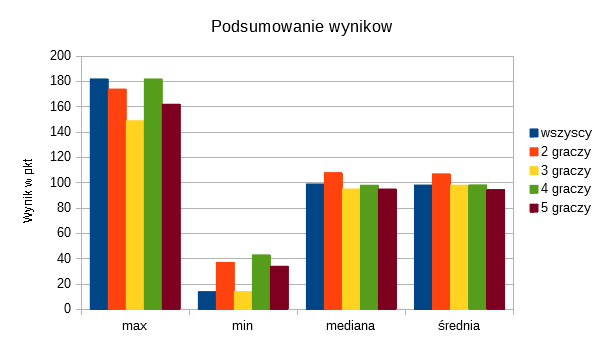
\includegraphics{WynikWPkt.png}
	\caption{Wyniki wg. ilości graczy}
	\label{figure:min_max_algo}
\end{figure}
\section{Wnioski i podsumowanie} 
Podsumowując otrzymane dane możemy dojśc do kilku wniosków, przede wszystkim, że decyzje podejmowane przez gracza komputerowego sprawiają wrażenie rzeczywistych. Gracz algorytmiczny ma swoje słabe oraz mocne strony po powoduje, że wykres częstości wartości punktów na koniec rozgrywki przypomina rozkład Gaussa. \\ \\
Zgodnie z wynikami wskazanymi w Tablicy \ref{table:algo_sizeresult} możemy zauważyć, że przewidywany wynik gracza powinien wynieść ok. 98 puntków (średnia oraz mediana). Wynik ten potwierdza przebieg wykresu z Rysunku \ref{figure:global_points_algo}, którego \textit{szczyt} znajduje się ok. 97-98 punktów. Można zauważyć, że spora część rozgrywek kończy się wynikiem powyżej 87 punktów. Powyżej wyniku 140 punktów znajduje się znikoma część graczy - według tablicy zaledwie 1,17\%. \\ \\ 
Wnioski możemy również wynieść z Rysunku \ref{figure:player_points_algo}, który wskazuje rozkład punktów w zależności od ilości graczy. Zgodnie z oczekiwaniami przebieg każdego z wykresu przedstawia rozkład Gaussa. Najlepsze wyniki osiągają gracze uczestniczący w rozgrywce dwuosobowej. Jest to spowodowane powolnym zapełnianiem planszy przez co zdobywają mniejszą ilośc punktów karnych za niezrealizowane bilety. W przypadku takiej konfiguracji można oczekiwać wyniku ok. 107 punktów. \\ \\ 
Bardziej zbliżone do siebie są rozgrywki trzy- oraz cztero-osobowe, dla których średni wynik wynosi 98 pkt. Można zauważyć, że dla rozgrywek trzyosobowych po osiągnięciu maksimum częstości, częstośc występowań wyników o danej ilości punktów maleje szybciej od rozgrywek czteroosobowych. Skutkiem tego jest znacznie wyższy procent graczy z wynikiem końcowym ponad 120 oraz ponad 140 punktów, co przedstawiono w Tablicy \ref{table:algo_sizeresult}.. \\ \\
Kolejnym zauważalnym wnioskiem są lepsze wyniki dla rozgrywek 2 oraz 4 osobowych niż 3 oraz 5 graczowych. Można to zauważyć w \ref{figure:min_max_algo}, gdzie w przypadku średniej oraz mediany jest zauważalny trend malejący wyniku względem ilości graczy. Jako przyczynę tej sytuacji można wskazać szybsze zapełnianiem się planszy. Można zaobserwować róznież niską średnią ilość niezrealizowanych biletów - można wnioskować, że co najmniej co drugi gracz zrealizował wszystkie swoje bilety. W kwestii zrealizowanych biletów ogólna średnia powyżej 3 biletów świadczy, że gracze zazwyczaj dociągali karty biletów. \\ \\
Wysoka amplituda wyników jest spowodowana dużym spektrum możliwych stanów planszy (rezerwacji połączeń, biletów oraz celów graczy), przez co możliwe są wyniki bardzo dobre (powyżej 140 punktów) jak i złe (poniżej 60). 
\chapter{Model sieci neuronowej}
\section{Wprowadzenie do eksperymentu}
Z łatwością można wskazać działanie przygotowanego algorytmu, gorzej jest w przypadku sieci neuronowej. Sieci neuronowe w swojej charakterystyce mogą być nieprzewidywalne, a duże znaczenie w jej efektywności odgrywa odpowiednie przygotowanie modelu danych, następnie struktury sieci a w końcu są potrzebne odpowiednie dane, które pozwolą sieć wyuczyć. \\ \\
Przygotowanie sztucznej inteligencji opartej o uczenie maszynowe dla tego typu zagadnień wydaje sie ciekawym podejściem. W większości gier uczestnik rozgrywki ma okrojony zakres dozwolonych w danym momencie typów decyzji (w algebrze  \textit{klas równoważności}). Przygotowanie klasyfikatora, którego celem będzie określenie jaka jest najlepsza w danym momencie decyzja jest realizowalne przez klasyfikator działający na podstawie uczenia maszynowego (np. DNNClassifier z biblioteki \textit{tensorflow}). Przygotowanie algorytmu, który wybierze odpowiednią decyzję niesie za sobą skutek w postaci rozbudowy algorytmu o dodatkowe rozgałęzienia i ujęcie przypadków szczególnych lub ograniczenie się do dobrego działania w okrojonego zakresu. Przygotowanie sieci neuronowej może pozwolić na obsługę zdarzeń szczczególnych - zwłaszcza w przypadku, gdy takie zdarzenie znajdzie się w zbiorze danych uczących.
 \\ \\ W przypadku gier planszowych, przygotowanie modelu danych nie jest niewykonalnym zadaniem, gdyż sama rozgrywka odbywa się w postaci unormowanej - większość zdarzeń oraz stanów możemy przedstawić w matematycznej formie - jako wartości / zmienne. W pierwszym kroku pracy nad siecią neuronową należało zbudować taki model danych w oparciu o \textit{Stan gry}, na podstawie którego sieć będzie mogła podjąć jednoznaczną decyzję. Model danych powinien być pozbawiony szumu w postaci zbędnych danych.
 \\ \\ Po przygotowanie modelu przystąpiono przygotowania danych uczących w oparciu o model algorytmiczny. Ostatnim krokiem przed rozpocząciem uczenia sieci było przygotowanie konfiguracji sieci, która będzie osiągać najlepsze wyniki w symulowanych rozgrywkach.
\section{Model danych wejściowych}
Model danych wejściowych przedstawiono w Tablicy \ref{table:algo_input}. W trakcie przygotowania kierowałem się danymi jakie są wykorzystywane w trakcie wyboru decyzji w algorytmie \textit{klasycznym}

\begin{longtable}[h]{| c | c | c | p{6.5cm} |} \hline
	Nazwa & Typ & Zakres & Opis \\ \hline	
	Tura & Int & 0-100 & Aktualna tura gracza \\ \hline
	Karty wagonów & Int & 0-120 & Suma kart wagonów gracza (wszystkich kolorów) \\ \hline
	Wagony na planszy & Int & 0-5 & Ilość wagonów na planszy \\ \hline
	Wagony w talii & Int & 0-120 & Ilość wagonów w talii \\ \hline
	Wagony odrzucone & Int & 0-120 & Ilość odrzuconych wagonów \\ \hline
	Bilety gracza & Int & 0-30 & Ilość biletów posiadanych przez gracza \\ \hline
	Bilety w talii & Int & 0-30 & Ilość biletów pozostających w talii \textit{biletów} \\ \hline
	Wagony gracza & Int & 0-45 & Ilość wagoników posiadanych przez gracza \\ \hline
	Punkty gracza & Int & -50 - 200 & Ilośc punktów posiadanych przez gracza \\ \hline
	Pozostałe karty wagonów & Int & 0 - 120 & Ilość kart wagonów w talii oraz na planszy  \\ \hline
	Liczba połączeń do zrealizowania & Int & 0 - 40 & Ilość połączeń na planszy, które gracz może zarezerwować \\ \hline
	Liczba połączeń pasujących & Int & 0 - 40 & Ilość połączeń, które gracz może zrealizować z trasy biletów. \\ \hline
	Liczba połączeń targetowych & Int & 0 - 40 & Ilość połączeń na trasie biletów. \\ \hline
	Liczba połączeń brakujących & Int & 0 - 40 & Ilość połączeń jakie brakuje graczowi do zrealizowania wszystkich biletów \\ \hline
	Liczba graczy & Int & 2-5 & Ilość graczy w rozgrywce \\ \hline
	Min wagonów  & Int & 0 - 45 & Najmniejsza liczba wagonów wśród pozostałych graczy \\ \hline
	max wagonów  & Int & 0 - 45 & Największa liczba wagonów wśród pozostałych graczy \\ \hline
	avg wagonów  & Int & 0 - 45 & Srednia liczba wagonów wśród pozostałych graczy  \\ \hline
	Mediana Wagonów & Int & 0 - 45 & Mediana liczby wagonów wśród pozostałych graczy  \\ \hline
	Min biletów & Int & 0 - 45 & Najmniejsza posiadanych liczba biletów wśród pozostałych graczy  \\ \hline
	max biletów & Int & 0 - 45 & Największa posiadanych liczba biletów wśród pozostałych graczy  \\ \hline
	avg biletów & Int & 0 - 45 & Srednia liczba posiadanych biletów wśród pozostałych graczy  \\ \hline
	med biletow & Int & 0 - 45 & Mediana liczba posiadanych biletów wśród pozostałych graczy  \\ \hline
	ticket fail & Int & 0 - 30 & Liczba biletów \textit{niezrealizowanych} przez aktywnego gracza \\ \hline
	ticket done & Int & 0 - 30 & Liczba biletów \textit{zrealizowanych} przez aktywnego gracza \\ \hline
	points for others & Int & 0 - 30 & Liczba punktów bez liczenia punktów za bilety \\ \hline
\caption{Dane wejściowe sieci neuronowej}
\label{table:algo_input}
\end{longtable}

\section{Model danych wyjściowych}
W eksperymencie wykorzystano klasyfikator, który operuje na pięciu możliwych klasach wyjściowych (do podglądu w \ref{table:algo_classifcator}):
\begin{table}[h]	
	\begin{center}
		\begin{tabular}{| c | c | c |} \hline
			\# & Nazwa & Opis decyzji \\ \hline
			0 & Opuszczenie tury & Gracz nie może podjąć żadnej decyzji \\ \hline
			1 & Pobranie karty wagonów & Gracz powinien pobrać karty tego typu (akumulacja zasobów) \\ \hline
			2 & Pobranie karty biletów & Gracz powinien pobrać karty tego typu (dobranie celów) \\ \hline
			3 & Zarezerwowanie połączenia & Gracz powinien zabezpieczyć punkty \\ \hline
		\end{tabular}
		\caption{Klasy określane przez klasyfikator}
		\label{table:algo_classifcator}
	\end{center}
\end{table}
\section{Struktura sieci}
W pracy wykorzystano klasyfikator oparty o pracę głębokich sieci neuronowych. Warstwa wejściowa składała się z 26 featerów. Następnie były dwie warstwy ukryte, które składały się odpowiednio z 160 oraz 120 neuronów. Na wyjściu klasyfikacja opierała się na 5 neurach.
\section{Proces weryfikacji uczenia}
W trakcie zbierania pomiarów kilkukrotnie zmieniano model danych. Sieć podejmowała często zabronione decyzje spowodowane wpływem niepotrzebnych \textit{featerów}. W związku z tym usunięto dane o poczynaniach innych graczy, a dodano ilość różnych kolorów kart wagonów posiadanych przez gracza oraz największą ilość kart tego samego koloru. \\ \\ 
Drugą ważną zmianą w modelu sieci neuronowej była redukcja ilości dozwolonych decyzji (klas). Początkowo jako punkt wejściowy był zapisany stan \textit{start}, lecz ostatecznie został on usunięty.
\section{Zbiór danych uczących}
Jak kilkukrotnie wspomniano w pracy jako zrodło danych uczących wykorzystano uruchomienie modelu algorytmicznego i zapis rozgrywek do pliku. Z powodu dużej amplitudy wyników zdecydowałem się na redukcję zbioru uczącego do zapisu trzydziestu parti (preferowane były jak najlepsze wyniki) dla każdej konfiguracji liczby graczy. 
\section{Wyniki} 
Wyniki otrzymane w trakcie eksperymentu zostały zawarte w Tablicy \ref{table:nn_sizeresult}, oraz ziilustrowane na wykresach \ref{figure:player_points_nn}, \ref{figure:global_points_nn} oraz \ref{figure:min_max_nn}.

\begin{table}[h]
	\begin{center}
		\begin{tabular}{| c | c | c | c | c | c |} \hline
			Cecha & 2 graczy & 3 graczy & 4 graczy & 5 graczy & ogólnie \\ \hline
			Minimum & 55 & 37 & 27 & 15 & 15 \\ \hline
			Maksimum & 163 & 178 & 159 & 180 & 180 \\ \hline
			Srednia & 106,41 & 100,01 & 100,13 & 96,23 & 99,69 \\ \hline
			Mediana & 107 & 100 & 101 & 98 & 101 \\ \hline
			(\%) > 110 & 38,07 & 38,27 & 24,79 & 21,12 & 25,71 \\ \hline
			(\%) > 120 & 14,81 & 10,24 & 10,12 & 7,54 & 9,92 \\ \hline
			(\%) > 140 & 2,26 & 0,55 & 1,14 & 0,79 & 1,05 \\ \hline
			Zrealizowane bilety & - & - & - & - & - \\ \hline
			Niezrealizowane bilety & - & - & - & - & - \\ \hline
			Ruchy zabronione & 7&9&8&22&46 \\ \hline
		\end{tabular}
		\caption{Wyniki uzależnione od ilości graczy}
		\label{table:nn_sizeresult}
	\end{center}
\end{table}

\begin{figure}[h]
	\includegraphics{NNWykrespunktow.png}
	\caption{Rozkład punktacji wg. ilości graczy}
	\label{figure:player_points_nn}
\end{figure}

\begin{figure}[h]
	\includegraphics{NNWykrespunktowglobal.png}
	\caption{Globalny rozkład punktów}
	\label{figure:global_points_nn}
\end{figure}

\begin{figure}[h]
	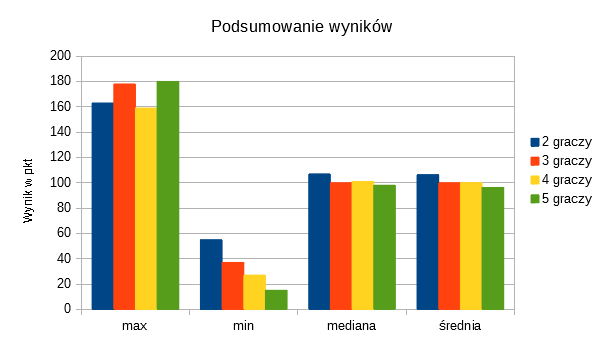
\includegraphics{NNWynikWPkt.png}
	\caption{Wyniki wg. ilości graczy}
	\label{figure:min_max_nn}
\end{figure}

\section{Podusmowanie}
Wyniki otrzymane w części dotyczącej sieci neuronowych wskazują, że proces uczenia miał swoje słabe i mocniejsze strony. Analogicznie do modelu algorytmicznego wraz z wzrostem ilości graczy model radził sobie coraz gorzej. Widać to zwłaszcza w mierniku \textit{Ruchy zabronione}, który oznacza, że sieć wskazała decyzję, która w danej turze była niemożliwa do zrealizowania. Najwięcej takich sytuacji zaszło w przypadku rozgrywek dla 5 graczy. \\ \\
W porównaniu do algorytmu, sieć radzi sobie znacznie lepiej w rozgrywkach od trzech do pięciu graczy jednocześnie nieznacznie tracąc w rozgrywkach dwuosobowych. Należy zaznaczyć, że średnia jest wyższa o 1,5 punktu zwycięstwa podczas gdy mediana aż o 2 punkty. Lepsza średnia jednocześnie została poniesiona kosztem rozgrywek o bardzo dobrym wyniku. Porównując Rysunki \ref{figure:global_points_algo} oraz \ref{figure:global_points_nn} można zauważyć, że w przypadku rezultatów rozgrywek sieci neuronowej rozkład jest bardziej śpiczasty, bardzo szybko rośnie częstość danego wyniku do maximum ok. 107 punktów. Następnie znacznie w porównaniu do modelu algorytmicznego szybciej spada. \\ \\
Kolejną zauważalną analogią są bardzo zbliżone do siebie wyniki rozgrywek trzy oraz czteroosobowoch. W analizie konfiguracji trend malejącej średniej oraz mediany się utrzymuje. Może zaskoczyć natomiast, że największe wyniki otrzymywane były w rozgrywkach 3 oraz 5 osobowych co możemy zaobserwować na \ref{figure:min_max_nn}. \\ \\
Na \ref{figure:player_points_nn} możemy natomiast zauważyć przebieg rozkładu punktów w zależności ilości graczy. Dla rozgrywek pięciograczowych wykres zaczyna rosnąć najwczęsniej, w okolicach 62 punktów zwycięstwa. Dla rozgrywek dla dwóch graczy wyniki zaczynają się czesciej pojawiać dopiero od poziomu 83 punktów, i jednoczęśniej najbardziej się wybijają. Z dwóch pozostałych konfiguracji, ta dla czterech graczy ma bardziej ostry przebieg. \\ \\
\section{Wnioski na temat uczenia}
Zgodnie z podstawami uczenia maszynowego - dużo zależy od tego jakie dane oraz w jakiej formie są dostarczone do sieci, którą chcemy nauczyć. Ograniczenia, jakie pojawiają się w przypadku zbioru danych uczących oraz słabości samych danych odbijają się na działaniu sztucznej sieci neuronowej. \\ \\ 
Lepsze średnie wyniki są spowodowane tym, że jako zrodlo danych do zbioru uczacego wykorzystano zapisy partii z najwyższą zdobyczą punktową. Pozwoliło to jednocześnie zachować schematy działania z originalnego algorytmu co zaskutkowało wymagającą w kontekście konfrontacji zdobyczą punktową. Niestety nie udało się doprowadzić do sytuacji w której nie zostały podjęte decyzje klasyfikowane jako zabronione. 
\chapter{Optymalizacja / Generalizacja}
\section{Wprowadzenie do eksperymentu}
Sztuczna inteligencja powinna w swoim działaniu dążyć do jak najlepszych wyników. W przypadku sztucznej sieci neuronowej najlepsze wyniki uzyskujemy poprzez dobór odpowiednich modelów / zbioru danych uczących. W przypadku sztucznej inteligencji dla rozważanej gry możemy:

\begin{enumerate}
	\item Przygotować specjalny model dla każdego konfiguracji liczby graczy, każdy model ma swój zbiór danych uczących. W dalszej części pracy nazwany \textbf{model specyficzny}
	\item Przygotować zaagregowany zbiór danych uczących z poprzedniego podpunktu. Model wykorzystywany jest w rozgrywkach niezależnie od konfiguracji. W dalszej cześci pracy nazwany \textbf{model uniwersalny}
\end{enumerate}

\section{Przebieg doświadczenia}
Na początku przygotowałem zbiory danych uczących dla każdej konfiguracji liczby graczy wybierając rozgrywki według najlepszego wyniku końcowego. Każdy zbiór danych składał się z zapisu decyzji trzydziestu graczy. Dodatkowo na końcu wszystkie zbiory danych uczących zapisane zostały do dodatkowego pliku \textit{all}, który zostaje wykorzystany do budowy modelu \textit{uniwersalnego}. \\ \\
Po przygotowaniu zbiorów danych uczących uruchomione zostało doświaczenie. Na początku przeprowadzenie uczenie sieci - 40 epok z rozmiarem batch'a 250 decyzji gracza. Dla każdej konfiguracji przeprowadzono po 60 rozgrywek - oddzielnie dla modelu uniwersalnego oraz modelu specyficznego. W sumie dla tej części przeprowadzono 480 gier testowych, których wyniki zamieszczono poniżej.
\section{Wyniki}
Wyniki otrzymane w doświadczeniu zostały zawarte w Tablicach \ref{table:nn_single_test} oraz  \ref{table:nn_all_test} oraz omówione w następnej sekcji.
\begin{table}[h]
	\begin{center}
		\begin{tabular}{| c | c | c | c | c | c |} \hline
			Cecha & 2 graczy & 3 graczy & 4 graczy & 5 graczy & ogólnie \\ \hline
			Minimum & 41 & 48 & 46 & 41 & 41 \\ \hline
			Maksimum & 157 & 140 & 148 & 142 & 157 \\ \hline
			Srednia & 101,66 & 99,4 & 97,36 & 92,05 & 96,57 \\ \hline
			Mediana & 99,5 & 101 & 100 & 91 & 97 \\ \hline
			Ukończonych rozgrywek & 60 & 55 & 60 & 56 & 231 \\ \hline
			(\%) > 110 & 28,33 & 24,24 & 25,00 & 18,57 & 23,11 \\ \hline
			(\%) > 120 & 18,33 & 10,30 & 8,75 & 8,21 & 10,31 \\ \hline
			(\%) > 140 & 4,17 & 0,00 & 0,42 & 0,36 & 0,87 \\ \hline
			Zrealizowane bilety & 467 & 575 & 873 & 951 & 2866 \\ \hline
			Niezrealizowane bilety & 63 & 66 & 102 & 135 & 366 \\ \hline
		\end{tabular}
		\caption{Podsumowanie - modele operujące na precyzyjnych danych uczących}
		\label{table:nn_single_test}
	\end{center}
\end{table}

\begin{table}[h]
	\begin{center}
		\begin{tabular}{| c | c | c | c | c | c |} \hline
			Cecha & 2 graczy & 3 graczy & 4 graczy & 5 graczy & ogólnie \\ \hline
			Minimum & 45 & 49 & 54 & 37 & 37 \\ \hline
			Maksimum & 154 & 133 & 144 & 143 & 154 \\ \hline
			Srednia & 108,12 & 96,51 & 97,69 & 94,88 & 98,00 \\ \hline
			Mediana & 108 & 97 & 99,5 & 96,5 & 99 \\ \hline
			Ukończonych rozgrywek & 60 & 60 & 59 & 56 & 235 \\ \hline
			(\%) > 110 & 43,33 & 24,44 & 23,73 & 21,07 & 25,86 \\ \hline
			(\%) > 120 & 25,00 & 7,78 & 8,05 & 7,14 & 10,17 \\ \hline
			(\%) > 140 & 3,33 & 0,00 & 1,27 & 0,71 & 1,10 \\ \hline
			Zrealizowane bilety & 515 & 603 & 855 & 939 & 2912 \\ \hline
			Niezrealizowane bilety & 41 & 90 & 83 & 111 & 325 \\ \hline
		\end{tabular}
		\caption{Podsumowanie - modele operujące na uniwersaslnych danych uczących}
		\label{table:nn_all_test}
	\end{center}
\end{table}
\section{Omówienie wyników}
Ciężko wskazać, które z dwóch sprawdzanych podejść odnosi lepsze rezultaty. Za kluczowe wskaźniki można uznać średni wynik oraz medianę punktów. Oba wskaźniki są wyższe w przypadku modelu uniwersalnego. Dodatkowo bardziej korzystna jest ilość dokonanych ruchów zabronionych. Na korzyść jest również w każdym przypadku procentowa ilość graczy, którzy przekroczyli podaną ilość punktów. Z drugiej strony model specyficzny ma niższy najniższy wynik oraz wyższy najwyższy wynik. \\ \\ 
Do ciekawszych wniosków prowadzą wyniki poszczególnych konfiguracji liczby graczy. Dla dwóch graczy uniwersalny (wspólny) model danych uczących daje znacząco lepsze rezultaty. Oczekiwana wartość punktowa jest wyższa aż o 7 punktów a w dodatku procentowy udział graczy z uzyskaną liczbą punktów wyższą od 110 punktów jest wyższy o 15 punktów procentowych. 
\\
\textbf{Rekomendacja: Model uniwersalny} \\ \\ 
Odwrotną sytuację można zauważyć w konfiguracji dla trzech graczy, gdzie sieć wyuczona danymi precyzyjnymi jest znacząco lepsza. Srednia zdobycz punktowa jest wyzsza o 3 punkty zwycięstwa a w dodatku wyższy jest odsetek graczy z końcowym wynikiem powyżej 120 punktów. 
 \\
\textbf{Rekomendacja: Model precyzyjny} \\ \\
Dla kolejnej z konfiguracji możemy zauważyć zbliżone do siebie wyniki. Zarówno średnia jak i mediana wyników są bardzo zbliżone do siebie - 97,36 oraz 97,69. Procentowy udział wyników powyżej 140 punktów jest lepszy dla uniwersalnych danych uczących. Dla zwiększenia prawdopodobieństwa uzyskania wyniku powyżej 110 oraz 120 punktów należało wykorzystać model precyzyjny. 
\\ \textbf{Rekomendacja: model precyzyjny} \\ \\ 
Ostatnią konfiguracją jest rozgrywka dla pięciu graczy. W tym przypadku lepsze wyniki osiągane są w przypadku modelu wyuczonego na uniwersalnych danych. Oczekiwana oraz mediana wyniku są wyższe o odpowiednio 2,83 oraz 5,5 punktów. Procentowy udział rozgrywek z wynikiem 110 oraz 140 punktów również działa na korzyść omawianego modelu. Dodatkowo, znacznie niższa jest liczba niezrealizowanych biletów. \\ \textbf{Rekomendacja: model uniwersalny} \\ \\
\section{Podsumowanie}
Podsumowując aktualny rozdział nie można jednoznacznie określić, z którego z tych dwóch modeli lepiej będzie skorzystać. Najlepiej będzie wykorzystać system mieszany, który adaptowalny byłby dla danej sytuacji. Dla rozgrywek dwu i pięcu osobowych wykorzystać model uniwersalny, dla pozostałych - model precyzyjny. Jako przyczynę przewagi w uogólnieniu - modelu uniwersalnego - można wskazać większą ilość różnych zdarzeń w trakcie rozgrywki. Dla graczy grających zgodnie z algorytmem dla konkretnej konfiguracji gry zakres  zdarzeń będzie ograniczony. Na przykład w rozgrywkach trójosobowych znacznie szybciej zapełnia się plansza, więc rozgrywka musi być przeprowadzona szybciej. Dlatego dla granicznych konfiguracji lepsze będzie wykorzystanie modelu uniwersalnego. W przypadku rozgrywek 3 i 4 osobowych, konnieczne będzie eliminacja jakiegokolwiek błędu, dlatego każdy ruch powinien być przemyślany, precyzyjny. 
\chapter{Dowód działania sieci}
\section{Wprowadzenie do eksperymentu}
Poza wskazaniem, że wyniki osiągane przez sieć neuronową są zbliżone do tych osiąganych przez algorytm należy udowodnić, że przygotowany model oraz założenia są słuszne. W tym celu określono metryki za pomoca których można opisać wyniki pracy sieci. Należy wskazać przede wszystkim, że wyniki osiągane w rozgrywkach sterowanych przez \textit{Losową} sieć neuronową są średnio gorsze od tych wyuczonych przykładowymi danymi.
\section{Model eksperymentu}
W celu udowodnienia działania modelu przeprowadziłem eksperyment w formie ewaluacji modelu w trakcie uczenia sieci. Dla każdej epoki składającej się z próbki pięciuset \textit{entry} przeprowadziłem ewaluację modelu dla losowych 100 wpisów z zbioru uczącego a następnie rozgrywałem sześćdziesiąt partii w każdej konfiguracji (od dwóch do pięciu graczy) co ostatecznie daje wynik 240 rozgrywek na iterację. Ilość danych uczących rośnie wraz z iteracją uczenia.
\section{Wyniki}
Wyniki otrzymane w trakcie doświadczenia umieszczono w Tablicy \ref{table:learn_metrics}.

\begin{figure}
	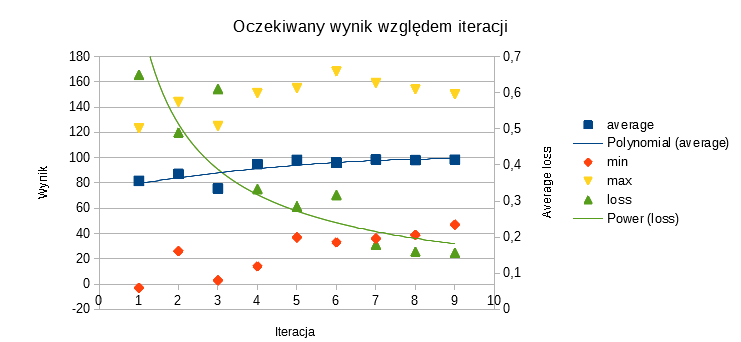
\includegraphics{WykresPunktowPosteIteracji.png}
	\caption{Rozkład punktacji w procesie uczenia}
	\label{figure:learn_results}
\end{figure}

\begin{table}[h]
	\begin{center}
		\begin{tabular}{| p{6cm} | c | c | c | c | c |} \hline
			Aktualna iteracja & 0 & 1 & 2 & 3 & 4 \\ \hline
			Sumaryczna ilość danych uczących & 0 & 100 & 200 & 300 & 400 \\ \hline
			Srednie odchylenie od próbki & 7.614 & 0.649 & 0.490 & 0.610 & 0.333 \\ \hline
			Srednia pewnosc klasyfikacji & 0.107 & 0.689 & 0.800 & 0.692 & 0.885 \\ \hline
			Liczba gier zakończonych przerwaniem (ruchem zabronionym) & 240 & 1 & 32 & 4 & 47 \\ \hline
			Maksymalna liczba punków & - & 123 & 144 & 125 & 151 \\ \hline
			Minimalna liczba punktów & - & -3 & 26 & 4 & 47 \\ \hline
			Liczba graczy która ukończyła rozgrywki & 0 & 835 & 702 & 824 & 654 \\ \hline
			Srednia zdobycz punktowa & - & 81.63 & 87.23 & 75.69 & 94.80 \\ \hline
			Srednia liczba tur potrzebnych do zakonczenia rozgrywki & 1.70 & 40.75 & 42.23 & 39.44 & 44.25 \\ \hline
			Srednia liczba ukonczonych biletów & - & 2,21 & 2,39 & 1,9 & 3,08 \\ \hline
			Srednia liczba nieukonczonych biletow & - & 0,43 & 0,33 & 0,54 & 0,32 \\ \hline
		\end{tabular}	
		\caption{Wyniki pierwszych pięciu epok uczenia}
		\label{table:learn_metrics}
	\end{center}
\end{table}

\section{Podsumowanie}
W dowodzie pojawia się trudność w ocenie postępów uczenia, gdyż rozważany problem nie jest trywialny i realna możliwość oceny sztucznej inteligencji pojawia się dopiero po rozegraniu całej partii trwającej średnio ok. 40 tur. \\ \\
Najprostszym wyznacznikiem jest średnia zdobycz punktowa, która dla losowej konfiguracji nie skutkowała żadną rozegraną do końca rozgrywką. W każdej z 240 gier, jeden z graczy dokonał ruchu zabronionego. Dosyć szybko, gdyż po zaledwie jednej epoce gracz komputerowy był w stanie rozegrać partię do końca. Na 240 gier zaledwie jedna zakończyła się podjęciem decyzji zabronionej. Niestety oczekiwany wynik uzyskiwany przez tą sieć był względnie niski. Dla modelu algorytmicznego oczekiwana wynosiła 98,16 (W nawiązaniu do Tablicy \ref{table:algo_sizeresult}), w tym przypadku wynik był aż o ok. 17 punktów niższy. Niskie wartości miały również najniższy osiągnięty wynik jak i najwyższy wynik w całej serii rozgrywek. \\ \\
Nie można wskazać dominującego trendu w dalszym procesie uczenia. Do szóstej iteracji uczenia (próbka danych uczących - 600) średnia wartość wyników gracza reguranie wzrastała. Od piątej epoki oczekiwany wynik wynosił ok. 95 punktów, co można uznać za akceptowalny wynik w kontekście zbioru uczącego. \\ \\ W trakcie procesu uczenia wzrastał natomiast najniższy osiągany wynik przez wszystkich graczy w wszystkich seriach testu. Natomiast wynik najwyższy utrzynywał się w granicach 150-160 punktów, który to wynik sprawiłby trudność doświadczonemu graczowi. \\ \\
Dodatkowo, na podstawie rysunku \ref{figure:learn_results} można zauważyć trend - rosnąca średnia wartość zdobyczy punktowej wraz z malejącą wartością sredniej straty (parametr average loss). Na wykresie można dostrzec również powolną stabilizację najwyższego oraz najniższego wyniku, jaki osiągnęła sięć w trakcie symulacji gier.
\chapter{Podsumowanie pracy}
Przygotowanie sztucznej inteligencji dla gry \textit{Wsiąść do pociągu} było jednoczesnie wyzywające oraz uczące. Do skutecznego działania konieczne było opracowanie algorytmów działajacych jednocześnie efektywnie jak i uniwersalnie. Jako cel założono uzyskanie jak najwyższego oczekiwanej wyniku z możliwością wybicia się przy odpowiednim ułożeniu kart. \\ \\ 
Dla redukcji złożoności problemów zrezygnowano z następujących elementów:
\begin{enumerate}
	\item Dodatkowe dziesięć punktów dla posiadacza najdłuższej ścieżki
	\item Interakcje polegające na blokowaniu sobie połączeń
\end{enumerate}
oraz założono, że gracz zawsze stara się grać jak najlepiej dla swojego wyniku. \\ \\  
Opisywana w pracy gra jest skomplikowana z dużą ilością danych, które opisać można jako losowe. Mamy do dyspozycje dwie różne talie - zasobów oraz biletów, problem grafowy oraz interakcje z innymi graczami. Trudnym zadaniem jest przygotować sztuczną inteligencję, która podejmie dobrą decyzję dla każdej decyzji, nawet tej najbardziej niszowej oraz nieprzewidywalnej. \\ \\ 
Otrzymane wyniki dowiodły, że zaproponowany algorytm może być wykorzystywany w trakcie rozgrywek oraz może posłużyć jako schemat działania, który można wykorzystać w własnych rozgrywkach. 
\chapter{Słownik}
\paragraph{Gracz}
Uczestnik rozgrywki - sterowany przez sztuczną inteligencję. Przygotowano poniższych uczestników
\subparagraph{Model algorytmiczny} Sztuczna inteligencja działająca w oparciu o algorytm. Wykorzystany do uzyskania danych uczących
\subparagraph{Sieć neuronowa} Sztuczna sieć neuronowa - klasyfikuje rodzaj decyzji jaka ma zostać podjęta przez gracza
\paragraph{Decyzja}
Podejmowana przez uczestnika rozgrywki decyzja (rezerwacja połączenia, pobranie kart wagonów lub pobranie kart biletów)
\subparagraph{Decyzja zabroniona}
Podjęta przez gracza decyzja niemożliwa w danym momencie z punktu widzenia gry. \textit{Przykładowo brakujące zasoby gry}
\paragraph{Bilet}
\label{dictionary:bilet}
Losowane przez uczestnika rozgrywki zadanie do zrealizowania. Określony przez dwa miasta, które gracz musi ze sobą połączyć (za pomocą zarezerwowanych połączeń). W przypadku udanego zrealizowania zadania gracz zdobywa określoną liczbę punktów. W przeciwnym przypadku punkty są odejmowane z zdobytej puli.
\paragraph{Połączenie}
Połączenie dwóch sąsiadujących ze sobą miast. Połączenia charakteryzują się ilością nitek (1 lub dwie), kolorystyką (jeden z 8 kolorów lub połączenie bezbarwne) oraz długością. Można zbudować graf wykorzystując miasta jako węzły oraz połączenia jako krawędzie.
\paragraph{Wagon} Element (w fizycznej wersji gry) służący do znakowania zarezerwowanych połączeń. Jeden wagonik odpowiada jednej karcie wagonów służacej do zarezerwowania połączenia. Gracz na początku posiada 45 wagonów. W momencie, gdy jeden z graczy ma 2 wagony lub mniej gracze wykonują jeszcze po jednym ruchu po czym przechodzą do fazy podliczenia punktów na koniec rozgrywki.
\paragraph{Karta wagonu} Element rozgrywki. W grze występuje jako jeden z 8 zasobów (kolorów) - po 10 sztuk, oraz karta joker (zastępuje dowolną kartę zasobów) - w ilości 12 sztuk. Gracz wykorzystuje karty zasobów do zrealizowania połączenia.
\paragraph{Stan gry} Stan rozgrywki składający się z informacji o planszy (w tym kolejność ułożenia niewidocznych kart) oraz informacji o graczach. Stan gry jest przedstawiony w sposób reduntantny - np. wagony przedstawione są jako licznik, a kolor gracza nie ma znaczenia - jedynie jego identyfikator.
\paragraph{Punkt (zwycięstwa)} Jest to wynik gracza. Punkt zwycięstwa zdobywa się za realizację biletów oraz rezerwacje połączeń między miastami.
\chapter{Bibliografia}
\begin{enumerate}
	\item{Instrukcja do gry}
	\subitem (Dostęp: ) \\ \url{https://www.wydawnictworebel.pl/repository/files/instrukcje/WdP_USA.pdf}
	\item{Omówienie botów do gry - forum Board Game Geek}
	\subitem (Dostęp: ) \\ 
	\url{https://boardgamegeek.com/thread/1523665/ai-project-solo-multiplayer-games}
	\item{Repozytorium projektu}
	\subitem(Dostęp: ) \\ \url{https://github.com/paqaos/msc-ticket-to-ride-nn-ai}
	\item{Algorytmy}
	\subitem Cormen
\end{enumerate}
\listoffigures
\listoftables
\end{document}